\documentclass{article}
\usepackage[utf8]{inputenc}
\usepackage[spanish]{babel}
\usepackage{listings}
\usepackage{graphicx}
\graphicspath{ {images/} }
\usepackage{cite}

\begin{document}

\begin{titlepage}
    \begin{center}
        \vspace*{1cm}
            
        \Huge
        \textbf{Nociones de la memoria del computador}
            
        \vspace{0.5cm}
        \LARGE
        Proyecto de investigación
            
        \vspace{1.5cm}
            
        \textbf{Juan Andres Urbiñez Gómez}
            
        \vfill
            
        \vspace{0.8cm}
            
        \Large
        Departamento de Ingeniería Electrónica y Telecomunicaciones\\
        Universidad de Antioquia\\
        Medellín\\
        Septiembre de 2020
            
    \end{center}
\end{titlepage}

\tableofcontents
\newpage

\section{Introducción}
El computador posee distintos tipos de memoria, cada una con su función y disponen de su capacidad solo para algo especifico, sabemos que todas tienen distintas arquitecturas en cuanto a cercanía del procesador se refiere, lo que lleva a que tengan menor o mayor capacidad para guardar información, haciendo que unas sean mas rápidas que otras 
\section{Definición de memoria del computador}
La memoria del computador se podría definir \cite{Augusto} como dispositivo donde se almacena información ya sea volátil o no volátil para luego ser llevada al procesador, estos usualmente su capacidad y velocidad son opuestamente proporcionales, es decir, a mayor capacidad, menor velocidad y viceversa.
\section{Tipos de memoria conocidas anterior a investigación} 
Antes de hacer esta investigación solo conocía muy pocos tipos de memoria siendo, RAM, cache, y el disco duro.

\subsection{Memoria RAM}\label{RAM}
Random Acess Memory o por sus iniciales <<RAM>> (Figura \ref{fig:ram}) en pocas palabras es la que toma parte de información del disco duro de algún proceso activo en el computador, y almacenarlo temporalmente para luego procesarlo. Al ser memoria temporal, al apagar el computador la información en la RAM  desaparece.

\begin{figure}[h]
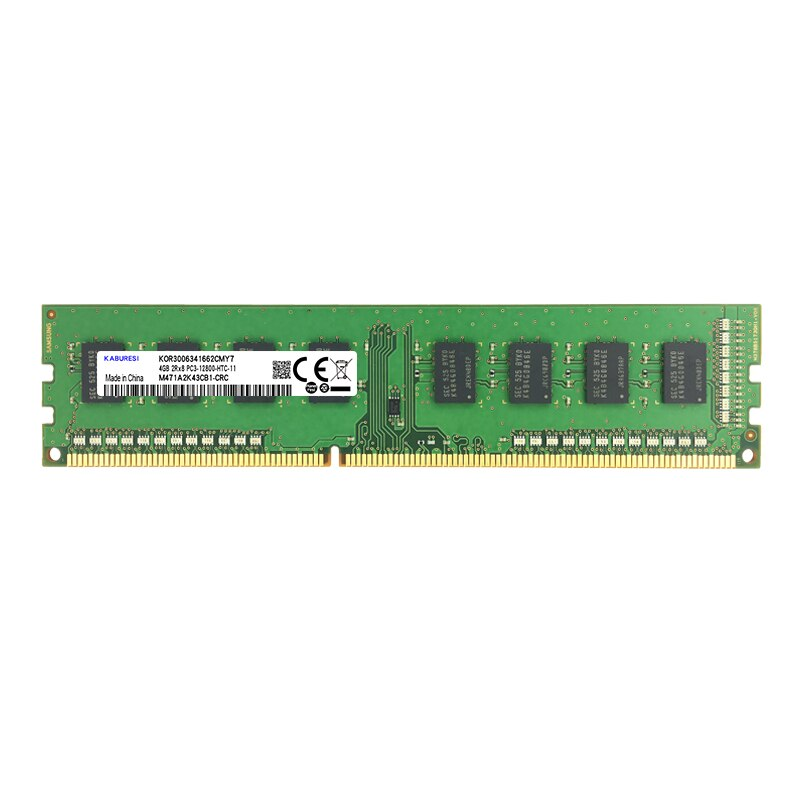
\includegraphics[width=4cm]{Images/Ram.jpg}
\centering
\caption{Memoria RAM}
\label{fig:ram}
\end{figure}

\subsection{Memoria cache}\label{cache}
La memoria cache a diferencia de la <<RAM>> esta muy cerca de la CPU (tanto que usualmente las CPU vienen con la memoria cache) para que la información requerida por la CPU llegue manera inmediata esta hay 3 tipos de memoria cache L1, L2, Y L3, donde L1 es la mas cercana a la CPU y L3 la mas alejada, en cuanto a capacidad $L1 < L2 < L3$.



\subsection{Disco duro}\label{discodurotxt}
El disco duro (Figura \ref{fig:discoduro}) es donde se almacena toda la información del computador que a diferencia de la RAM, en este no se pierde al apagarlo.

\begin{figure}[h]
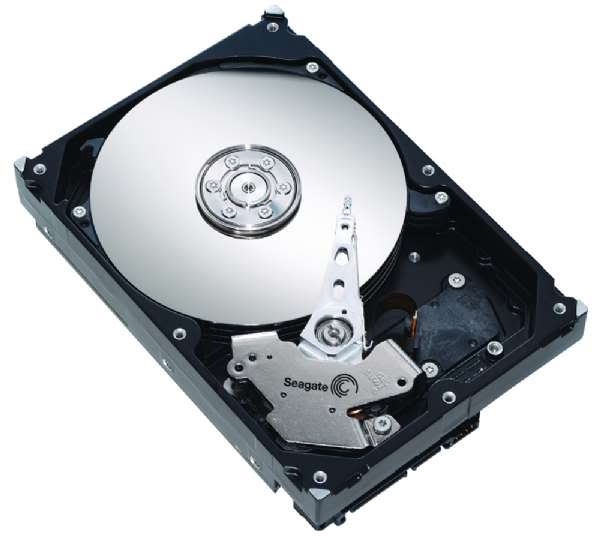
\includegraphics[width=4cm]{Images/discoduro.jpg}
\centering
\caption{Disco duro}
\label{fig:discoduro}
\end{figure}

\section{Gestión de memoria en el computador}

La gestión de memoria es el procedimiento que asigna y libera espacios de memoria en la RAM realizado por el Memory Management Unit (Figura \ref{fig:MMU})  para que sea usado por los programas en ejecucion, de esto esta encargado el controlador de memoria  ubicado en la motherboard.
\cite{UdManizales} Una vez terminado el proceso el controlador se encarga de guardar los cambios en el disco duro y liberar la informacion de la RAM para quede libre y se le pueda asignar otros procesos.

\begin{figure}[h]
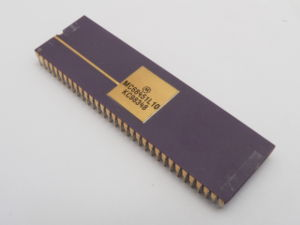
\includegraphics[width=4cm]{Images/MMU.jpg}
\centering
\caption{Memory Managment Unit (MMU)}
\label{fig:MMU}
\end{figure}

\section{Memorias y su rapidez}

\subsection{¿Por qué la memoria en un computador son tantas?}
Hasta ahora hemos visto que hay varios tipos de memoria, el disco duro (Sección \ref{discodurotxt}) que se encarga de guarda información de manera ``permanente''
en el computador y tiene una gran capacidad en comparación a la RAM (Sección \ref{RAM}) que posee poca capacidad de información y esta cerca al procesador lo que hace que la información llegue al procesador mas rápido.

\vspace{0.5cm}

También hablamos de otro tipo de memoria llamada cache (sección \ref{cache}) esta al estar tan cerca del procesador y tener tan poca capacidad llega a ser muy rápida, por lo que podemos decir que la \textbf{velocidad} de la memoria \textbf{depende} de la \textbf{cercanía al procesador} y \textbf{capacidad de almacenamiento.}

\subsection{Importancia}
Gracias a la división de memorias en el computador el procesador siempre dispone de información para procesar y se saca el mayor rendimiento el dicho procesador, al necesitar información constantemente el procesador saca gran beneficio de la memoria cache estando tan cerca del procesador. \cite{Osan}de manera similar que la disco duro se beneficia de la RAM al tener menor capacidad y mayor cercanía al procesador.
\section{Conclusión} \label{conclulsion}
Después de conocer los tipos de memoria, como funcionan y sus debidas arquitecturas, entendemos porque funcionan y la importancia que tienen todas,sin el disco duro el computador no podría guardar ningún cambio que hagamos en el pc para usos posteriores y fuera incapaz de usar un sistema operativo propio, sin la RAM el computador no podría ejecutar ningún proceso, ya que en este es el que se encarga de mantener la información de los procesos en ejecución, de no ser por la memoria cache el procesador tendría grandes fallas de rendimiento, debido a que tiempo de viaje de la información de la RAM a la CPU no es el mismo que el cache a CPU.
\newpage
\bibliographystyle{IEEEtran}
\bibliography{references}

\end{document}

